%! TeX program = lualatex
\documentclass[12pt,a4paper]{instrukcja}

\begin{document}

\begin{center}
	\vspace*{2cm}

 	\hrulefill
	
	\vspace{0.7cm}
	

		\textbf{\textsc{{\Huge{Obrzędy Wielkiego Tygodnia}}\\\bigskip{\large wg OHS 1955-1962}}}
	
	\vspace{0.5cm}
	
	\hrulefill

	\vspace{\fill}	

	 {\large \textbf{Użyte oznaczenia:}} \\
	
	 \vspace{0.1\textwidth}
	 
	 {\large\centering
	   \begin{itemize}[leftmargin=.43\linewidth,rightmargin=.35\linewidth,label=]
	    \item \ii~ -- celebrans 
	    \item \dd~ -- diakon 
	    \item \ss~ -- subdiakon
 	    \item \cc~ -- ceremoniarze 
	    \item \aa~ -- akolici 
	    \item \tt~ -- turyferarz 
	    \item \ding{63} -- krzyż procesyjny
	    \item \oo -- ombrelino
	  \end{itemize}
	 }
	
	\vspace{5cm}	
	
	\hrulefill
	
	{\footnotesize Pierwsza edycja -- 9 kwietnia 2017\\
	Druga edycja -- 8 kwietnia 2019 \\
	Wszelkie zastrzeżenia proszę kierować do autora na adres: \texttt{michal96.96@gmail.com}}

	\newpage
\end{center}

	

\thispagestyle{empty}

\tableofcontents

% \newpage

\pagestyle{plain}

%! TeX program = lualatex
\documentclass[10pt,a4paper]{instrukcja}

\fancyhead{}
\fancyfoot[C]{Imprimatur 		-- ks. Ireneusz Bakalarczyk}
\fancyfoot[L]{Nihil Obstat		-- Jakub Gajewski}
\fancyfoot[R]{Skład 			-- Michał Siemaszko}

\begin{document}

%%%%%%%%%%%%%%%%%%%%%%%%%%%%%%%%%%

\header{Oczyszczenie NMP}
%%%%%%%%%%%%%%%%%%%%%%%%%%%%%%%%%%
\section{Poświęcenie Gromnic i procesja}

\begin{itemize}
	\item Do prezbiterium wychodzimy normalnie, kapłan ubrany w białą kapę
	\item Po \textit{Dominus vobiscum} następuje 5 oracji po czym zasypanie,
	      pokropienie i okadzenie (potrzebny turyfer i ministrant z kropielnicą)
	      \footnote{\textbf{UWAGA}: może być tak, że celebrans pójdzie pokropić
		      świece wiernych}
	\item Świece rozdawane są ministrantom w sposób podobny do przyjmowania
	      Komunii Św.
	      \footnote{w trakcie rozdawania śpiewa się \textit{Pieśń Symeona}}
	\item Po zakończeniu rozdawania świec następuje ostatnia oracja
	\item Formuje się procesja z krzyżem i akolitami. Idą w niej wszyscy
	      ministranci, celebrans oraz  wierni. Wszyscy mają \underline{zapalone świece}.
	\item Idziemy dookoła kościoła i wracamy do prezbiterium
	\item Po powrocie celebrans zakłada biały ornat i wszyscy gaszą gromnice
\end{itemize}

\section{Zmiany na Mszy Świętej}

\begin{itemize}
	\item Brak modlitw u stopni ołtarza
	\item Msza z dnia bez perturbacji
	\item Zapalamy gromnice na Ewangelię i od \textit{Sanctus} do końca Kanonu.
	\item Zaleca się zrobienie lucenarium
\end{itemize}

\end{document}


%! TeX program = lualatex
\documentclass[10pt,a4paper]{instrukcja}

\begin{document}

%%%%%%%%%%%%%%%%%%%%%%%%%%%%%%%%%%
\pagestyle{empty}

\header{Pasterka}
%%%%%%%%%%%%%%%%%%%%%%%%%%%%%%%%%%
\section{Procesja wejścia}

\begin{itemize}
	\item W kościele należy wygasić światła.
	\item Kapłan ubrany w kapę koloru białego bez akompaniamentu organów
	      się do żłóbka ustawionego w prezbiterium. (W tym czasie jeden z
	      usługujących może uderzyć 12 razy w gong)
	\item Po przyjściu kładzie figurkę Dzieciątka i przykrywa ją welonem.
	      Następnie staje przy krześle wraz z asystą.
	\item Kantor staje na ambonie i śpiewa Kalendę: \smallbreak
	      %
	      \inde{Octavo Kalendas Januarii Luna N.\\
		      Innumeris transactis saeculis a creatione mundi, quando in
		      principio Deus creavit caelum et terram et hominem formavit ad
		      imaginem suam;\\
		      permultis etiam saeculis, ex quo post diluvium Altissimus in
		      nubibus arcum posuerat, signum fœderis et pacis;\\
		      a migratione Abrahæ, patris nostri in fide, de Ur Chaldæorum
		      saeculo vigesimo primo;\\
		      ab egressu populi Israël de Ægypto, Moyse duce, saeculo decimo
		      tertio;\\
		      ab unctione David in regem, anno circiter millesimo;\\
		      hebdomada sexagesima quinta, juxta Danielis prophetiam;\\
		      Olympiade centesima nonagesima quarta;\\
		      ab Urbe condita anno septingentesimo quinquagesimo secundo;\\
		      anno imperii Cæsaris Octaviani Augusti quadragesimo secundo;\\
		      toto orbe in pace composito, \textbf{Jesus Christus}, æternus Deus
		      æternique Patris Filius, mundum volens adventu suo piissimo
		      consecrare, de Spiritu Sancto conceptus, novemque post
		      conceptionem decursis mensibus, in Bethlehem Judæ \textbf{nascitur
		      ex Maria Virgine factus homo}:}
	      \smallbreak
	\item[] Tu zapala się światła w kościele.
	      \smallbreak
	      \inde{Nativitas Domini nostri \textbf{Jesu Christi} secundum carnem.}
	      %
	\item Tu bije się we wszystkie dzwonki (podobnie jak w czasie
	      \textit{Gloria} w trakcie Wigilii Paschalnej) i odzywają się organy.
	\item Rozpoczyna się śpiew pieśni Wśród Nocnej Ciszy. Kapłan w tym czasie
	      odkrywa figurkę Dzieciątka, nakłada kadzidło do kadzielnicy i okadza
	      figurkę Dzieciątka. Można też teraz przyozdobić żłóbek kwiatami.
	\item Po zakończeniu śpiewu wszyscy siadają, a kapłan udaje się na ambonę i
	      wygłasza homilię.
	\item Po homilii kapłan ubiera szaty mszalne koloru białego i rozpoczyna
	      Mszę jak zwykle.
\end{itemize}

\section{Zmiany na Mszy Świętej}

\begin{itemize}
	\item Podczas lekcji imię \textbf{Jezus} pada dwa razy -- na oba razy
	      skłaniamy głowę w stronę krzyża
	\item Jeśli wystarczy ministrantów to robimy lucenarium
	\item Jest bożonarodzeniowe \textit{Communicantes}
\end{itemize}

%%%%%%%%%%%%%%%%%%%%%%%%%%%%%%%%%
\footer{
	Nihil Obstat	-- Karol Pyziołek 			\hfill 
	Imprimatur 		-- ks. Ireneusz Bakalarczyk \hfill 
	Skład 			-- Michał Siemaszko}
\end{document}


%\chapter{}

\section{Sposoby służenia na Piasku}

\subsection{Rodzaje Mszy Św.}

\begin{itemize}
	\item \textbf{recytowana} -- z jednym lub dwoma ministrantami
	\item \textbf{recytowana świąteczna} (także kolędowa) -- z jednym lub dwoma,
	      w niedziele i święta poza wielkim postem, klęczy się na niej i stoi
	      jak na mszy śpiewanej
	\item \textbf{śpiewana \textit{na dwóch}} -- msza śpiewana bez \cc~ i \tt~
	\item \textbf{śpiewana z okadzeniem} -- standardowa msza niedzielna z \cc~ i
	      \tt~
	\item \textbf{ śpiewana \textit{bardziej uroczysta}} -- bardziej uroczysta
	      msza świąteczna	(np. Wigilia Zesłania Ducha Św.), z lucenarium,
	      obrusem komunijnym, okadzeniem i ew. dodatkowymi obrzędami
	\item \textbf{solenna} -- z asystą \dd~ i \ss, lucenarium
\end{itemize}

\noindent Przy zastosowaniu bardziej uroczystych form liturgicznych -- jeśli
jest duża ilość ministrantów -- wyznacza się drugiego ceremoniarza, który
\begin{itemize}
	\item prowadzi procesję wejścia i inne procesje, które także ustawia przed
	      wyruszeniem. Dba o dobre tempo
	\item wprowadza duchownych i ministrantów do chóru
	\item w razie potrzeby zajmuje miejsce przy \cc1, aby wspólnie asystować
	      \ii.
	\item kontroluje na bieżąco, czy czegoś nie brakuje, czy nie powinien czegoś
	      donieść itp.
	\item wprowadza lucenarium i procesję „dwójkami” do przyjmowania Komunii Św.
\end{itemize}


\section{Poświęcenie palm i procesja}

\begin{itemize}
	\item w tej części \dd~ wykonuje pocałunki \ii~ standardowo jak podczas mszy
	\item podczas ubierania (na {\color{red} czerwono}) celebransa asystuje \cc,
	      kolejno diakona \aa1 oraz subdiakona \aa2
	\item ustawiamy się w szyku procesyjnym. \dd~ i \ss~ przez cały czas
	      procesji i poświęcenia ,jeżeli jest to możliwe, trzymają kapę.
	      Wychodzimy przez główne wyjście na zewnątrz. Przy przechodzeniu przez
	      oś ołtarza polowego, przyklękają wszyscy oprócz: \ding{63}, \aa1, \aa2
	      oraz \ii
	\item schola śpiewa podczas procesji \textit{Hosanna filio David} na
	      przemian z Psalmem 117 \footnote{Zob. \textit{Liber Usualis} z 1961 :
		      Ritus servandus in celebratione Missae in Cantu ad 1.}
	\item po dojściu na miejsce święcenia palm, \cc~ odbiera nakrycia głowy,
	      następuje  oddanie referencji ołtarzowi przez \dd~ i \ss~ oraz \ii~
	      (\dd~ i \ss~ przyklękają, \ii~ głęboko się skłania), \ii~ całuje
	      ołtarz następnie ustawiamy się w sposób przedstawiony na Rys.
	      \ref{fig:przyjscie}

	      \begin{figure}[h]
		      \centering
		      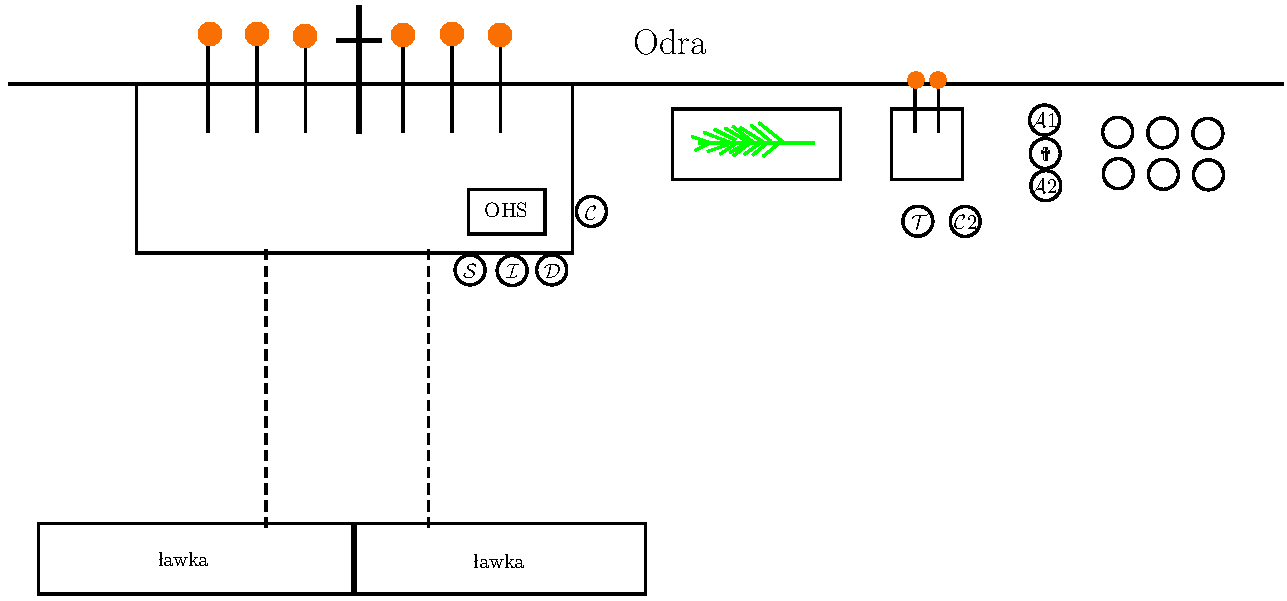
\includegraphics[width=0.8\linewidth]{Palmowa/PalmyNadOdra.pdf}
		      \caption{Ustawienie po przyjściu do ołtarza}
		      \label{fig:przyjscie}
	      \end{figure}

	\item \ii~ cicho odczytuje antyfonę \textit{Hosanna filio David}, tak jak
	      podczas Mszy, a następnie śpiewa \textit{Dominus vobiscum}, zwrócony w
	      kierunku księgi
	\item po \textit{Amen} następuje zasypanie
	\item \aa1 podaje wodę \cc~ a ten podaje ją \dd
	\item następuje pokropienie, \aa1 odbiera wodę od \dd
	\item następuję okadzenie
	\item palmę dla \ii~ \dd~ kładzie na ołtarzu
	\item następuje rozdawanie palm (\cc2 podaje palmy, \cc1 zawiaduje ruchem),
	      odbieranie palm od \ii~ i \dd~ z pocałunkiem, asysta ustawia się
	      dwójkami jak do komunii w kolejności: \dd~ i \ss~, klerycy,
	      ministranci, lud
	\item po rozdaniu palm \ii~ i \dd~ myją ręce, pomagają mu w tym \aa\aa
	\item następuje odśpiewanie ewangelii, nie przenosi się mszału
	\item do ewangelii ustawiamy się jak podczas mszy, gdy już dojdziemy na
	      miejsce jak na Rys. \ref{fig:ewangelia}

	      \begin{figure}[h!]
		      \centering
		      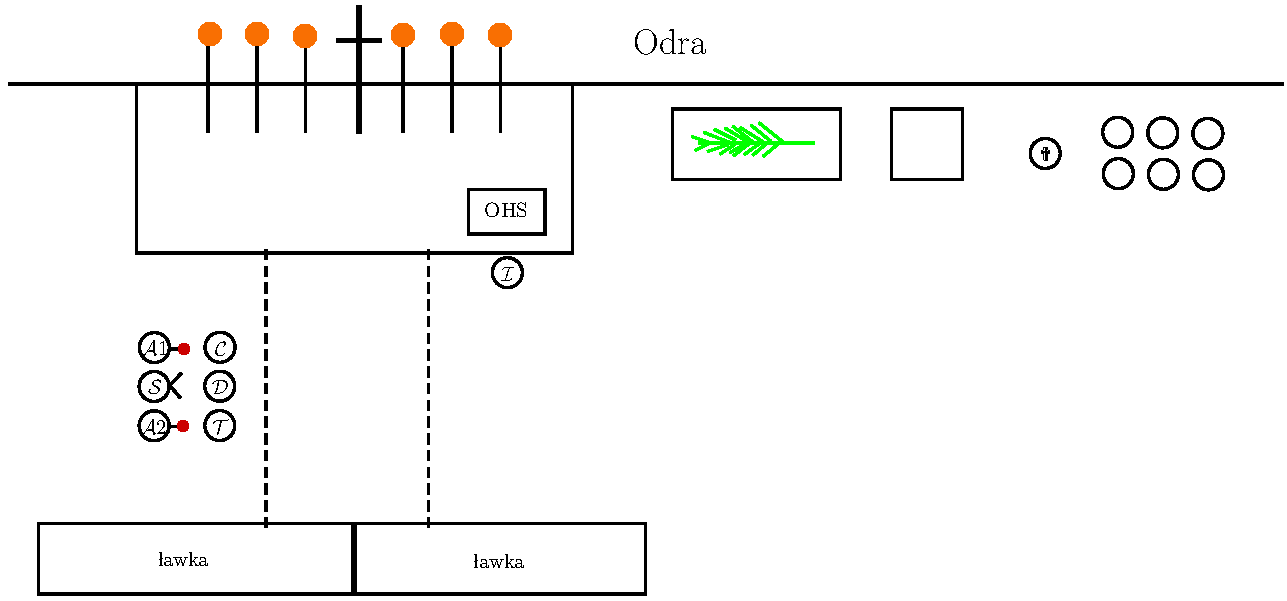
\includegraphics[width=0.8\linewidth]{Palmowa/PalmyNadOdra2.pdf}
		      \caption{Ustawienie podczas Ewangelii}
		      \label{fig:ewangelia}
	      \end{figure}

	\item po odśpiewaniu ewangelii \ii~ całuje ewangeliarz oraz jest okadzany
	      przez \dd
	\item kantorzy ($K1$) oraz mikrofoniarz udają się najkrótszą możliwą drogą
	      do pierwszych drzwi kościoła. Przymykają je lekko, ale obserwują, czy
	      procesja już się zbliża. Dwóch lub jeden kantor ($K2$) pozostaje w
	      procesji z ministrantami
	\item po powrocie do pozycji z Rys. \ref{fig:przyjscie} następuje zasypanie
	\item \dd~ i \ss~ stają w rzędzie za \ii
	\item \dd~ staje obok rzędu i śpiewa \textit{Procedeamus in pace}
	\item kantor ($K2$) oraz mikrofon wraz z ludem śpiewa \textit{In nomine
		      Christi. Amen}, a następnie rozpocznie jedno z poniższych:

	      \begin{itemize}
		      \item śpiew jednej z antyfon procesyjnych z \textit{Liber
			            Usualis}
		      \item \textit{Christus vincit}
		      \item pieśń po polsku do Chrystusa Króla
	      \end{itemize}

	\item po oddaniu rewerencji ołtarzowi \cc~ oddaje nakrycia głowy
	\item ustawiamy się w szyku procesyjnym, $K2$ zajmują w procesji miejsce
	      zaraz za \ding{63}
	\item udajemy się w kierunku bocznych drzwi po schodach za pomnikiem biskupa
	      Kominka
	\item $K1$ wewnątrz kościoła obserwują delikatnie, czy procesja nadchodzi
	\item kiedy procesja dochodzi do drzwi kościoła, \ss~ z \aa\aa~ stają przodem
	      do drzwi, a ministranci rozchodzą się na boki tworząc szpaler tak aby
	      \ii~ znajdował się nieopodal \ding{63}, jak na Rys. \ref{fig:procesja}

	      \medskip

	      \begin{figure}[h]
		      \centering
		      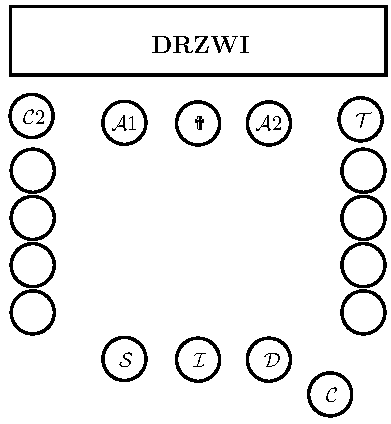
\includegraphics[width=0.26\linewidth]{Palmowa/PalmyNadOdra3.pdf}
		      \caption{Procesja przy drzwiach kościoła}
		      \label{fig:procesja}
	      \end{figure}
	      \todo{A gdzie mają być ci kantorzy na tym rysunku?}

	\item $K1$ (w środku) stojąc zwróceni w kierunku drzwi śpiewają:
	      \textit{Gloria Laus et honor} etc.
	\item $K2$, ministranci i wierni powtarzają werset: \textit{Gloria Laus}
	\item $K1$ śpiewają poszczególne zwrotki hymnu, po każdej zwrotce
	      $K2$ i reszta odśpiewują refren: \textit{Gloria, Laus}
	\item po piątej zwrotce i refrenie \ding{63} głośno i widocznie uderza nóżką
	      krzyża procesyjnego w drzwi, a $K1$ i \cc2 szeroko otwierają drzwi
	\item \cc2 wprowadza \ding{63} i resztę procesji do wnętrza kościoła. W tym
	      czasie $K1$ i $K2$ łączą się w jedną grupę i jak najszybciej zaczynają
	      śpiew: \textit{Ingrediente Domino}, podany w
	      \textit{Liber Usualis}
	\item \dd, \ss, \ii~ oraz \cc~ po przyklęknięciu na środku udają się
	      bezpośrednio do księgi po stronie epistoły, reszta asysty i chór
	      przyklękają po kolei na środku. Wszyscy zajmują swoje miejsca i
	      odkładają palmy. \aa\aa~ odkładają świece a \ding{63} krzyż na stojak
	\item modlitwa na zakończenie procesji od Mszału ustawionego przy ołtarzu po
	      stronie Epistoły, \dd~ i \ss~ trzymają brzegi kapy (jak przy poświęceniu)
	\item po skończonej oracji, \ii~ i \dd~ oraz \ss~ podchodzą do sedilli i
	      przebierają się (w {\color{violet}fiolety}). Przebieranie przebiega w
	      następującej kolejności:

	      \begin{itemize}
		      \item \cc~ zabiera kapę przekazuje \zz
		      \item \dd~ i \ss~ ściągają dalmatyki z pomocą \aa1 oraz \aa2
		      \item \cc~ ubierają w ornat \ii, \zz~ zabierają w tym
		            czasie dalmatyki i manipularze czerwone
		      \item \aa1 zakłada tunicelę \ss, \aa2 dalmatykę \dd
		      \item \cc~ sprawdza czy \dd~ i \ss~ mają odpowiednie szaty
	      \end{itemize}

	\item w czasie przebierania schola śpiewa \textit{Introit}
\end{itemize}

\section{Liturgia słowa}

\begin{itemize}
	\item po przybyciu do prezbiterium stajemy następująco:
	\item (tutaj będzie grafika)
	\item następuje zasypanie, potem \cc~ odmawia modlitwę, okadzenie księgi i
	      \textit{Exsultet}
	\item \aa~ biorą z kredensu świeczki i odpalają sobie, podobnie \mm1
	\item \cc2 na słowa \textit{O vere beata nox...} zapala lampy w
	      prezbiterium.
	\item po orędziu paschalnym \cc2 wraz z \aa2 pomagają \ii~ przebrać się z
	      powrotem w kapę
	\item następnie \cc~ odnosi dalmatykę do zakrystii i wraca na swoje miejsce
	      razem z drugim OHS
	\item \cc1 zabiera z pulpitu białą narzutkę i kładzie na pulpicie teksty
	      proroctw
	\item \ding{63} odnosi krzyż za ołtarz
	\item \tt~ odnosi kadzielnicę i wraca na swoje miejsce
	\item siedzimy w prezbiterium następująco:
	\item (tutaj będzie odpowiednia grafika)
	\item następują proroctwa
	\item po trzecim proroctwie \tt~ idzie po kadzielnicę i bokiem przemyka w
	      stronę chrzcielnicy i zapala tam światła
\end{itemize}

\section{Lucenarium}

\opis{Potrzebne: 6(4) ministrantów siedzących w chórze, \cc2 lub \tt~ (gdy nie
	ma \cc2 \tt~ prowadzi i daje znaki), 6(4) pochodni wystawionych koło bazy \tt}

\begin{itemize}
	\item Po okadzeniu ludu \tt~ zatrzymuje się n przy stopniu prezbiterium i
	      zwraca się w kierunku ołtarza. Dołącza do niego \cc2 i 6 ministrantów
	      wyznaczonych do lucenarium.
	\item Na znak \cc2 klękają i wychodzą do bocznej nawy po pochodnie.	(Rys.
	      \ref{fig:wyjscie})
	\item Przygotowują pochodnie, mogą zasypać kadzielnicę.
	\item Na śpiew \textit{Sanctus} bardzo powoli wchodzą do prezbiterium
	      rozchodząc się na boki (Rys.\ref{fig:wejscie_1})
	\item Ustawieni odpowiednio przyklękają, po czym klękają na dwa kolana
	      (Rys.\ref{fig:wejscie_2})
	\item \tt~ zajmuje miejsce z prawej strony na pierwszym stopniu ołtarza.
	      Klęczą przez cały Kanon.
	\item Na \textit{Per omnia saecula saeculorum} wstają, wykonują skłon na
	      \textit{Oremus}, a następnie przyklękają i na czele z \tt~ i \cc2
	      wychodzą z prezbiterium (Rys. \ref{fig:wyjscie_1} oraz Rys.
	      \ref{fig:wyjscie_2})
\end{itemize}

\begin{figure}[h]
	\centering
	\includegraphics[width=0.29\linewidth]{wyjscie}
	\caption{Wyjście ministrantów podczas ofiarowania}
	\label{fig:wyjscie}
\end{figure}

\begin{figure}[ht]
	\savebox{\imagebox}{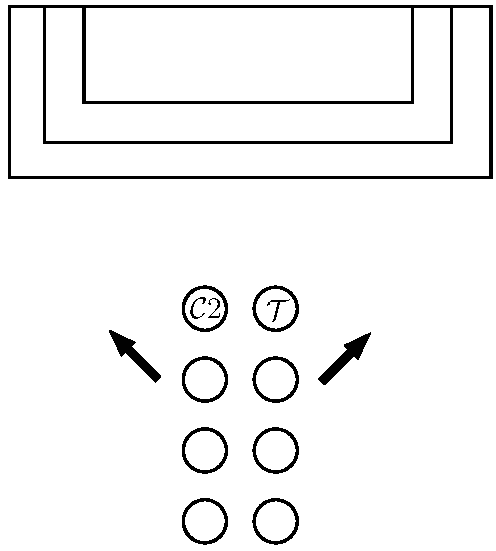
\includegraphics[width=.4\linewidth]{wejscie_1}}%
	\begin{subfigure}[t]{.5\linewidth}
		\centering\usebox{\imagebox}
		\caption{Przed przyklęknięciem}
		\label{fig:wejscie_1}
	\end{subfigure}\qquad
	\begin{subfigure}[t]{.5\linewidth}
		\centering\raisebox{\dimexpr\ht\imagebox-\height}{% Raise smaller image
			into place \includegraphics[width=\linewidth]{wejscie_2}}%
		\caption{Po przyklęknięciu}
		\label{fig:wejscie_2}
	\end{subfigure}
	\caption{Wejście ministrantów na \textit{Sanctus}}
\end{figure}

\newpage

\begin{figure}[ht]
	\savebox{\imagebox}{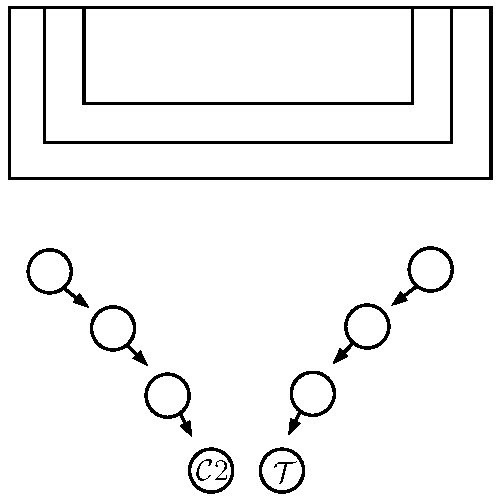
\includegraphics[width=.4\linewidth]{wyjscie_2}}%
	\begin{subfigure}[t]{.5\linewidth}
		\centering\raisebox{\dimexpr\ht\imagebox-\height}{% Raise smaller image
			into place 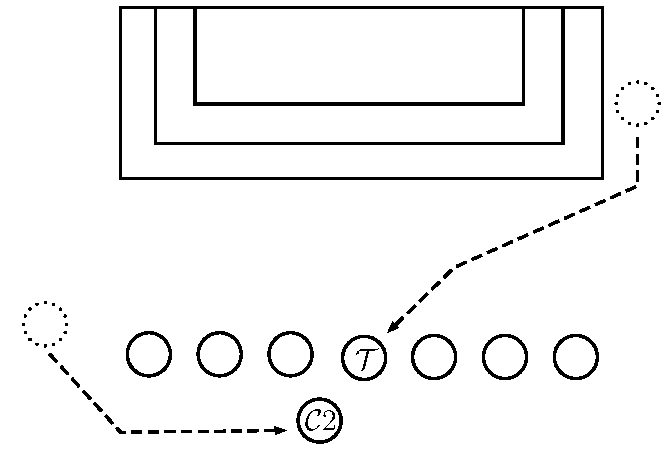
\includegraphics[width=\linewidth]{wyjscie_1}}%
		\caption{Przed przyklęknięciem}
		\label{fig:wyjscie_1}
	\end{subfigure}\qquad
	\begin{subfigure}[t]{.5\linewidth}
		\centering\usebox{\imagebox}
		\caption{Po przyklęknięciu}
		\label{fig:wyjscie_2}
	\end{subfigure}
	\caption{Wyjście ministrantów po \textit{Per omnia secula seculorum}}
\end{figure}

\textbf{Uwaga!} Na Mszy Wieczerzy Pańskiej w Wielki Czwartek ministranci z
pochodniami nie wychodzą z prezbiterium, tylko oczekują na procesję.

\section{Dodatek}

\subsection{Przebieg poświęcenia wody}
\label{sec:woda}
\begin{enumerate}
      \item \textit{Dominus Vobiscum} i Oracja 0. (przed wejściem)
            \smallfont{(złożone ręce)}
      \item \textit{Dominus Vobiscum} i Oracja 1. \smallfont{(złożone ręce)}
      \item Prefacja do słów \textit{Sumat unigeniti tui gratiam de Spiritu
                  Sancto}
      \item \ii~ kreśli znak krzyża
            \textcolor{red}{\raisebox{-1mm}{\scalebox{1.5}{\ding{64}}}} na
            wodzie
      \item Wyciera ręce
      \item Kontynuuje modlitwę
      \item Na \textit{Sit haec} kładzie rękę na powierzchni wody
      \item Wyciera rękę
      \item Kreśli znaki krzyża
            \textcolor{red}{\raisebox{-1mm}{\scalebox{1.5}{\ding{64}}}}
            nad wodą na słowa \textit{Per Deum vivum \dots}
            \vspace*{-11pt}
      \item Wylewa wodę na cztery strony świata po słowach \textit{... super te
                  ferebatur} ~~~
            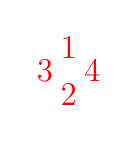
\begin{tikzpicture}[scale=0.3, baseline=-1mm, thick]
                  \draw[color=red] (10mm,0) node {\large 4};
                  \draw[color=red] (-10mm,0) node {\large 3};
                  \draw[color=red] (0,10mm) node {\large 1};
                  \draw[color=red] (0,-10mm) node {\large 2};
            \end{tikzpicture}
            \vspace*{-7pt}
      \item Kreśli znak krzyża nad wodą na \textit{Benedico te}
      \item Po zmianie głosu na \textit{recto tono} na słowa \textit{tu benignus
                  aspira} trzy razy dmucha do wody na kształt krzyża
      \item W tym czasie \cc1 podaje Paschał
      \item Na słowa \textit{Descendad in hanc} trzy razy wkłada Paschał do wody
            i śpiewa \footnote{Wkłada Paschał coraz głębiej}
      \item \ii~ trzy razy dmucha do wody w kształcie litery
            \textcolor{red}{\raisebox{-1mm}{\Large ${\Psi}$}} i kontynuuje
            \textit{Totamque ... effectu}
      \item Wyciągamy Paschał z wody i kończymy święcenie wody (\textit{... per
                  ignem.})
      \item Po \textit{Amen} nabiera się wody do pokropienia
      \item Pokropienie i \textit{Com przyrzekł Bogu \dots}
      \item Następnie \cc1 przynosi do chrzcielnicy tackę z olejami świętymi i
            wręcza \ii~ (z pocałunkiem) odpowiednie ampułki. \ii, wypowiadając
            słowa przepisane w księdze po kolei:
            \begin{itemize}
                  \item wlewa olej katechumenów
                  \item wlewa krzyżmo
                  \item wlewa oba
            \end{itemize}
      \item Następnie miesza wodę ręką lub przy pomocy łyżeczki \footnote{W
                  razie potrzeby myje i wyciera ręce; wykorzystuje sól, watę i
                  miękisz chleba, które później należy spalić. Wodę z tej
                  ablucji wlewa się do sacrarium.}
\end{enumerate}

\subsection{Bierzmowanie}
\label{sec:bierz}
\begin{enumerate}
      \item \dd~ i \ss~ podtrzymują kapę; księgę trzyma \cc1, a \cc2 stoi z boku
            przy kredencji
      \item \ii~ zwraca się do kandydatów \textit{Spiritus
                  Sanctus superveniat\dots Amen.}
      \item \ii~ żegna się mówiąc \textit{Adjutorium nostrum...}, potem krótki
            dialog
      \item \ii~ wyciąga ręce nad kandydatami i mówi
            \textit{Oremus. Omnipotens sempiterne Deus,\dots}
      \item Bierzmowany klęka przed \ii. Świadek kładzie rękę na
            prawym ramieniu bierzmowanego.
      \item \cc2 podchodzi do \dd~ z Krzyżmem Świętem
      \item \ii~ kładzie prawą rękę na głowie bierzmowanego i palcem umoczonym w
            Krzyżmie Świętym robi znak krzyż a na czole, mówiąc \textit{Signo te
                  signo\dots}
      \item \ii~ uderza lekko w policzek bierzmowanego, mówiąc \textit{Pax tecum}
      \item Bierzmowany wraca na swoje wcześniejsze miejsce i klęczy
      \item \cc2 odbiera Krzyżmo, i podchodzi z watą do wytarcia palców; później
            wraca do kredencji
      \item Gdy \ii~ namaści wszystkich kandydatów, śpiewa się antyfonę
            \textit{Confirma hoc, Deus\dots}
      \item Powtarza się antyfonę, a następnie \ii~ zwrócony do ołtarza śpiewa
            \textit{Ostende nobis, Domine,\dots}
      \item Następnie odwraca się do ludu i mówi \textit{Oremus. Deus, qui
                  Apostolis tuis\dots}
      \item \ii~ mówi \textit{Ecce sic benedicetur omnis homo, qui timet Dominum}
      \item Na końcu \ii~ błogosławi bierzmowanych
            \textit{Bene} \textcolor{red}{\raisebox{-1mm}{\scalebox{1.5}{\ding{64}}}}
            \textit{dicat vos Dominus ex Sion\dots}
\end{enumerate}

\color{red}

\section{Uwagi}
\begin{itemize}
      \item można zrobić jakieś święcenie ognia przed proroctwami tak aby ludzie
            oświetlali kościół i mieć jakąś namiastkę Wigilii Paschalnej
            \todo{raczej odpada}
      \item na poświęcenie wody ludzie \textbf{muszą mieć zapalne świece}
      \item zapytać księdza czy będzie aspersja (czy to humanitarne?)
            \todo{Będzie aspersja dla najbliżej stojących osób}
      \item ziomek do chrztu musi siedzieć za kratą aż do ochrzczenia -- trzeba
            mu przygotować jakieś krzesło i klęcznik \todo{jednak raczej nie bo
                  będzie to słabo wyglądało. Poza tym ziomek normalnie chodził na Msze
                  Św. na piasku więc czemu nagle nie może w nim być}
\end{itemize}

\end{document}
